\chapter{Fundamentals}
\label{chapter:fundamental}
In this first chapter, we lay out the fundamentals used in the rest of this thesis. At the beginning, we will introduce basic definitions such as \emph{utterance}, \emph{sample} and \emph{conversation}. We will then follow up with an introduction into machine learning using a special variant of \emph{Neural Networks} (NN), called \emph{Recurrent Neural Network} (RNN). We show the basic principles behind it and explain problems this RNNs have in practice, and how the can be solved by utilizing other forms of RNNs. We then show how RNNs can be used to build models, called \emph{Sequence-To-Sequence} (seq2seq) models \cite{Sutskever:2014}, which are capable of learning and using a language in a conversational context.

The following introduction only covers a small part of the spectrum of possibilities with regard to the tasks these models can perform. Basically, we are restricting our explanations to the supervised learning use-case and ignore the unsupervised ones, even though they have a wide area of applications (e.g. dimensionality reduction, regression) as shown by !REFERENZ FÜR UNSUPERVISED LEARNING?!. A basic introduction into the principles of neural networks can be found in appendix \ref{fundamentals:neural_networks}.

\section{Definitions}
\paragraph{Utterance} \blindtext
\paragraph{Sample} \blindtext
\paragraph{Conversation} \blindtext

\section{Recurrent Neural Networks}
\emph{Recurrent neural networks} (RNN) are a special variation of the NNs described in appendix \ref{fundamentals:neural_network}. The main difference between them is, that RNNs have a recurrence built into it, which allows them to adapt to problems which also have a temporal dimension and are dependent on data from differente timesteps to solve. We're also going into the problems such RNNs have due to their recurrence and how this problem can be solved by exploiting another form of RNN, called \emph{Long Short-Term Memory Networks} (LSMT).

\paragraph{RNNs in principle}
One of the main restrictions of vanilla NNs is the following: Assume a task, where the NN is conditioned to output a prediction on tomorrows weather given yesterdays. Now, if one would use a vanilla NN as described in the appendix, the main restriction would be that the NN has to make its prediction solely based on the weather information of the day before. Such a model does not take into account, that weather is not only dependent on the weather of the previous day, but also on the days before. This could be solved by feeding, say, the weather of the last week to the network instead of just the weather of the previous day. But if new scientific evident now shows, that weather is not only dependent on last week, but also on the last month, probably the last year, we quickly get into problems due to the sheer size of a NN performing such tasks, because the input size grows rapidly. Also, such a NN would still be static in the way, that one cannot simply change the time-window used to feed to the network. If one settles with one month, it will always be able predict the weather based on the last month, but not any different time-window, otherwise the NN has to be retrained using another time-window in order to work again as before. RNNs (see figure \ref{fundamentals:rnn:rolled_vanilla}) try to solve this problem by introducing a recurrence into the network, which allows it to exploit informations not only from the current input, but also from inputs of the past. In a more formal way, one could say that this recurrence allows RNNs to ''exhibit dynamic behaviour across the temporal dimension of the input data''.

\begin{figure}[h]
	\label{fundamentals:rnn:internal_structure}
	\centering
	\includegraphics[width=10cm]{img/rnn_internal}
	\caption{Internal structure of a vanilla RNN.\protect\footnotemark}
\end{figure}
\footnotetext{http://r2rt.com/static/images/NH\_VanillaRNNcell.png}

Before explaining how this recurrence can be used to solve the weather prediction problem, let's first show the equations used for the forward propagation in a RNN with a single cell. A single layer in an RNN is called a \emph{cell}. 

The internal structure is similar to the one of NNs, as explained in appendix \ref{fundamentals:neural_network}, except for the recurrence which we're going to elaborate on below.

\begin{equation}
\begin{split}
h_t & = \varphi_h(\mathbf{w}_h \cdot \mathbf{x}_t + \mathbf{u}_h \cdot \mathbf{h}_{t-1} + \mathbf{b}_h) \\
    & = \varphi_h\bigg(\sum_{i=0}^{n} w_i x_{ti} + \sum_{i=0}^{n} u_i h_{t-1i}\bigg)
\end{split}
\label{fundamentals:rnn:forward_equation:hidden}
\end{equation}

\begin{equation}
\begin{split}
o_t & = \varphi_y(\mathbf{w}_o \cdot \mathbf{h}_t + \mathbf{b}_o) \\
    & = \varphi_y\bigg(\sum_{i=0}^{n} w_i x_{ti} + \sum_{i=0}^{n} u_i h_{t-1i}\bigg)
\end{split}
\label{fundamentals:rnn:forward_equation:output}
\end{equation}

In the equations above, one can see different variables with different indices which we'll explain briefly:

\begin{itemize}[noitemsep]
	\item $x_t$ stands for the input at time-step $t$.
	\item $o_t$ stands for the output of the network at time-step $t$.
	\item $h_t$ stands for the hidden state at time-step $t$.
	\item $\mathbf{w}_h$, $\mathbf{w}_o$ and $\mathbf{u}$ are the weight matrices learnt while training the model.
	\item $\mathbf{b}_h$ and $\mathbf{b}_o$ stand for the bias vectors used when computing the new hidden state or output respectively.
	\item $\varphi_y$ and $\varphi_h$ are the activation functions used to compute $o_t$ and $h_t$ respectively.
\end{itemize}

As seen above, at every time step $t$, the new hidden state $h_t$ and the output $o_t$ are computed. The value of $o_t$ can be seen as the prediction of the RNN at time step $t$ and the value of $h_t$ is the value that is passed to the same cell in the next time step $t+1$ for computing the next output $o_{t+1}$ (and hidden state $h_{t+1}$). As depicted in figure \ref{fundamentals:rnn:internal_structure}, the hidden state $h_t$ is returned to the cell for computing the output $o_{t+1}$ and $h_{t+1}$. This is what an RNN allows to exhibit behaviour depending on data seen in past time steps: It can ''remember'' what it has already seen and the information necessary for the prediction in the hidden state, which is passed along the temporal dimension when a RNN is run through multiple steps in time.

To come back to our weather prediction problem, this allows the cell to remember what weather it has seen in the past (e.g. rainy, sunny, high pressure, low pressure) and adjust its future predictions accordingly. The recurrence also solves the problem of time windows of differente sizes: Since the recurrence allows the model to store the required informations in the hidden state at each time step and combine it with what it has already seen to make future predictions, it is not constrained to a fixed size of inputs required to make a prediction but instead uses all information it has already seen, no matter if the seen information is from the past 5 days or past 5 years, it can compress all this into the hidden state $h_t$.

While this is the solution for our problem of different window sizes, it is also a main bottleneck of the model: If one imagines, that the time window is past information is 5 years and we process these informations on a daily basis, we would need to remember the informations from around 1800 days. If we would now have 10 distinct features per day, this leads to 18'000 features to ''remember'' in total. Remembering means to ''compress'' the information into the hidden state, which is usually much smaller than 18'000, reasonable values vary from 128 up to 4096, depending on the structure and complexity of the problem. Another obstacle is, that the RNN cell has no way of ''forgetting'' informations stored in the hidden state easily, as the equation \ref{fundamentals:rnn:forward_equation:hidden} only does an addition to the hidden state $h_{t-1}$. Of course, in theory it is still possible that the RNN learns to forget insignificant informations, but this is a really hard problem in practice, why we are going to introduce yet another form of RNN cells, called \emph{Long Short-Term Memory} cells, which not only solves this problem, but also the problem of vanishing and exploding gradients explained in the next paragraph.

\paragraph{Vanishing / Exploding Gradient Problem} The recurrent nature of RNNs can cause problems in practice, one of the most problematic is the vanishing/exploding gradients problem: While training such networks, we condition the weight matrices $\mathbf{w}_h$, $\mathbf{w}_o$ and $\mathbf{u}$ via backpropagation by using gradient-descent in such a way, that the loss function is minimized w.r.t. to these parameters for the given training samples. This means, that we have to compute the derivates of the loss function by using the chain-rule $\frac{dz}{dx} = \frac{dz}{dy}\frac{dy}{dx}$. The entirety of all derivations w.r.t. to the parameters is called the gradient. Since the gradient also flows through the activation functions $\varphi_h$ of the recurrence, this computations also include the derivations of this function. Most of the commonly used activation functions today have codomains in $\mathbb{R}$ and take on values in the range of $[-1, +1]$ (e.g. $\operatorname{tanh}$), this means that multiplying a lot of this derivate values possibly leads to an exploding or vanishing values. This has a severe effect on training the RNN: If the value of the derivates is exploding, this means that the weights are adjusted in a way which we would call ''hyperbolism'' and this leads to a network where the predictions get worse and worse. On the other hand, if the values are vanishing, the network stops learning from a certain point in time on, since the weights are not really adjusted anymore, but only updated with tiny values which don't have any impact.

The problem of vanishing gradients was first analyzed by Sepp Hochreiter in his diploma thesis !!REFERENZ!!. A more formal explanation of the problem with links to dynamic systems and formal proofs, under which conditions these problems occur, can be found in \cite{Pascanu:2013}. The details on how backpropagation with gradient-descent is adapted to RNNs and time-dependent problems, called \emph{Truncated Backpropagation Through Time} or \emph{TBTT} in short, can be found in \cite{Werbos:1990}.

\paragraph{Long Short-Term Memory Networks} To solve the problem with vanishing/exploding gradients mentioned before, J\"urgen Schmidhuber and Sepp Hochreiter introduced an advanced version of a RNN cell, called \emph{Long Short-Term Memory}, or LSTM in short \cite{Hochreiter:1997}. The structure of this kind of cells is much more sophisticated then vanilla RNN cells, but it also solves the two most pressing problems: Vanishing/Exploding gradients and the inability to forget stored information.

It does this by introducing the so-called \emph{gates} into the cell, which are nothing else than small NNs which are responsible for deciding which informations from the previous time step we are going to keep in the old hidden state $h_{t-1}$, add to the new hidden state $h_t$ and use for the computation of the output $o_t$. There are three different gates in an LSTM cell (as depicted in figure \ref{fundamentals:lstm:internal_structure}):

\begin{itemize}
	\item \textbf{Input gate}: Is responsible to decide which part of the input is interesting and should be used to update the hidden state $h_{t-1}$ to become the new one $h_t$.
	\item \textbf{Forget gate}: Is responsible to decide which part of the hidden state $h_{t-1}$ the cell is going to forget.
	\item \textbf{Output gate}: Decides which part of the hidden state $h_t$ is used to compute the output $o_t$.
\end{itemize}

\begin{figure}[h]
	\label{fundamentals:lstm:internal_structure}
	\centering
	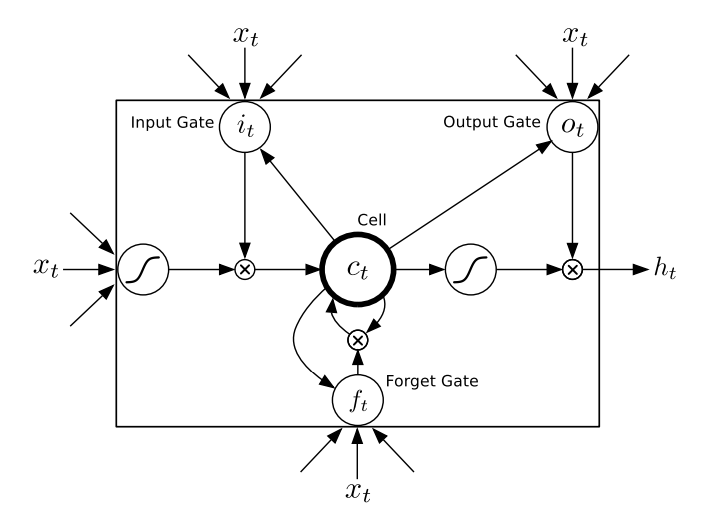
\includegraphics[width=10cm]{img/lstm_internal}
	\caption{Internal structure of a LSTM cell.\protect\footnotemark}
\end{figure}
\footnotetext{http://suriyadeepan.github.io/2016-12-31-practical-seq2seq/}

In theory, these gates do nothing more good than a plain RNN cell. However in practice this structure solves all of the aforementioned problems to at least some degree.

First, let us look into the vanishing/exploding gradient problem: The problem occured due to the fact, that the derivation of the activation function for the recurrence is used when calculating the updates of the weight parameters by performing backpropagation with gradient-descent. This can lead to vanishing (if the derivate is below 1) or exploding (if the derivate is above 1) gradients. The LSTM cell solves this problem by not applying an activation function on the recurrence, but rather using the identity function $f(x) = x$ whose derivation is always $1$. This practically solves this problem because the gradients can neither explode nor vanish.

The second problem is that an RNN cell has no easy way of forgetting information stored in the hidden state. This is obviously solved by the introduced gates which allow the cell to decide at each time step $t$, which information to keep, forget and store based on the last hidden state $h_{t-1}$ and the current input $x_t$. With this structures in place, the LSTM cell is able to track long-term dependencies much better than a vanilla RNN cell.

There are more details regarding the LSTM cell, like the forget bias and peephole connections, which can be looked up in a empirical study by Greff et al. \cite{Greff:2016}. There are even more architectures for RNN cells like \emph{Gated Recurrent Unit} \cite{Chung:2014} and \emph{Convolutional LSTM} \cite{Xingjian:2015}, which we will not go in depth on in this thesis.

\section{Sequence-To-Sequence Learning}
The RNN and LSTM cells described in the preceeding chapter can now be used to build so-called \emph{Sequence-To-Sequence} (seq2seq) models. They were first introduced by Sutskever et al. \cite{Sutskever:2014} as a generic model for learning to map arbitrary input to output sequences. They have shown, that such models can be successfully adapted to machine translation tasks and exhibit almost state-of-the-art performance. For more general informations on where and how seq2seq models can be leveraged we refer to chapter \ref{related_work}. In the following paragraphs, we are going to explain the basic idea behind the model and how each of its parts, called encoder and decoder, work when applied to conversational modeling.

\paragraph{Model}
The basic idea behind the model is to separate the parts necessary to understand and parse the input sequence, called the \emph{encoder}, from the part that is responsible for generating the output sequence, called the \emph{decoder} (see figure \ref{fundamentals:seq2seq:internal_structure}). Both the encoder and decoder can be any kind of RNN cell, be it GRU, LSTM or any other kind. The encoder is fed with the input sequence through multiple time steps, as an example one could say that for example each word of an input sentence is fed to the encoder one at a time. Through this process, the encoder starts to build its internal hidden state and updates it every time a new word is fed. After the input sequence is fully processed by the encoder, it then passes the information collected in the hidden state, in the context of seq2seq models also called \emph{thought vector}, to the decoder cell. The decoder cell then uses this hidden state as its own, internal, initial state and starts to produce the output sequence, one token per time step, after its fed with a dedicated \texttt{GO} token (also depicted in figure \ref{fundamentals:seq2seq:internal_structure}). The tokens are produced by feeding the final state of the decoder cell to a softmax classification layer which outputs probabilities over the words in the vocabulary. It then usually chooses (when using a greedy decoding approach, see paragrahp ''Decoding Approaches'') the ''best'' token to output in a greedy fashion by simply selecting the token with the highest probability after the softmax layer has been applied. The details on how the decoding exactly works are described in the paragraph \emph{Decoding Approaches} below. In general, the decoder tries to construct a sensible answer given the thought vector it received from the encoder.

\begin{figure}[h]
	\label{fundamentals:seq2seq:internal_structure}
	\centering
	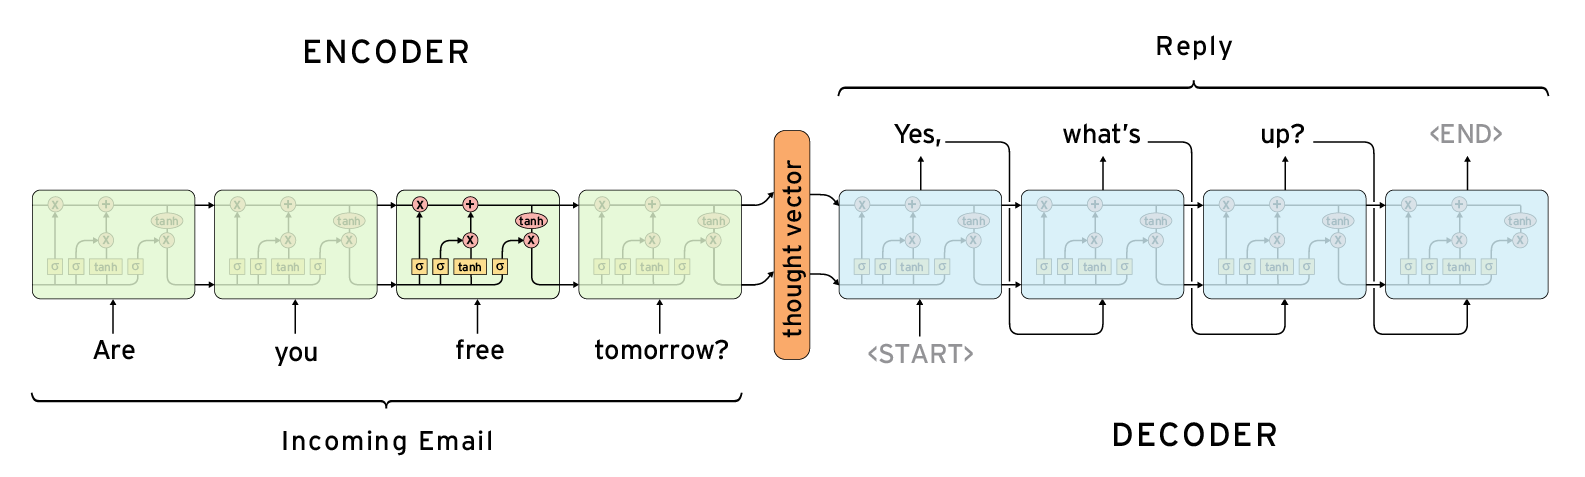
\includegraphics[width=12cm]{img/seq2seq_internal}
	\caption{Internal structure of a Sequence-To-Sequence Model.\protect\footnotemark}
\end{figure}
\footnotetext{http://suriyadeepan.github.io/2016-12-31-practical-seq2seq/}

Such a model is also called an \emph{end-to-end} model because it, beeing fully differentiable, can be trained by using backpropagation with gradient-descent with ease. The training works by having pairs of input-output samples which are then used to train the network and condition it to generate the expected output given the input sequence. This is done by feeding the network the expected words as inputs at each time step which allows for gradient-descent to be applied. Formally, if we're talking about language modeling, the model is conditioned to optimize the conditional probability $p(y_1,\dots,y_{t_1}|x_1,\dots,x_{t_2})$, where $t_1$ is the length of the input sequence and $t_2$ the length of the corresponding output sequence. As said before, the encoder cell produces a thought vector $t$, which is nothing more than its hidden state after it has processed the input sequence $x_1,\dots,x_2$, and passes this to the decoder for generating the output sequence. Hence, the following equation is a formal way of expressing the conditional probability such a model is trained to maximize:

\begin{equation}
p(y_1,\dots,y_{t_1}|x_1,\dots,x_{t_2}) = \prod_{t=1}^{t_1} p(y_t|t,y_1,\dots,y_{t-1})
\end{equation}

If we look at the example depicted in figure \ref{fundamentals:seq2seq:internal_structure}, the generation of the output sequence is done as follows:

\begin{enumerate}
	\item Feed the encoder with the current input word $x_t$ and update its hidden state accordingly. The output of the cell can be ignored.
	\item Repeat step 1 until the inputs $x_1,\dots,x_{t_1}$ are exhausted when $t_1$ is the length of the input sequence.
	\item Pass the hidden state of the encoder cell to the decoder cell after the first has processed the last word of the input sequence $x_{t_1}$.
	\item Initialize the decoder with the given hidden state and feed it the dedicated \texttt{GO} token.
	\item Store the output token $y_t$ of the decoder cell. After this, it depends on which decoding approach is used to generate the output sequence:
	\begin{enumerate}
		\item In case of a greedy decoder, simply feed the output $y_t$ back in to the decoder cell to produce the next output token $y_{t+1}$.
		\item If case of a beam-search decoder, select the $N$ outputs $y_1,\dots,y_{N}$ with the highest probability and store them. Feed each of this outputs back in to the decoder cell.
	\end{enumerate}
	\item Repeat step 5 until the decoder either outputs an \texttt{EOS} token or the maximum length $t_2$ for the output is reached.
\end{enumerate}

The concatenated outputs $y_1,...,y_{t_2}$ are the output of the model. The exact decoding approaches are described in more detail in the \emph{Decoding Approaches} paragraph below. Generally speaking, such models can be used for \emph{any} sequence-to-sequence problem, not just language modeling, as long as it is possible to define a probability distribution over the output tokens $y_t$ given the context $y_1,\dots,y_{t-1}$ and the thought vector $t$. The generality of this model has been shown several times !!REFERENZEN!!.

\paragraph{Soft-Attention Mechanism}
Imagine you have been asked to solve the following, simple task: Read a longer text about a certain topic. At the end of the text, there are several questions regarding this text and you have to answer them. How does a human approach such a task? Usually, most of the people start by reading the text through one time and then start to answer the questions. A normal human cannot remember the whole content of the text (since it is a long one), so what it does is to focus on a single question and try to find the answer by revisiting the text. This essentially means that the participant in this task \emph{focuses} their \emph{attention} on single parts of the text instead of the text as a whole. This is basically what the \emph{soft-attention} mechanism is all about. Let us adapt the introductory example on how this behavior could be adapted to seq2seq models and how it helps to solve tasks.

As mentioned before, the main bottleneck of seq2seq models is that the encoder has to compress all the information it has processed into its thought vector. The thought vector is then passed to the decoder which tries to come up with a meaningful answer to the information stored in the thought vector. If a long text is compressed into the thought vector, this might not be an easy task to solve as the information has to be compressed too much. The attention mechanism helps by solving this issue by allowing the decoder to ''look'' at all thought vectors of the encoder at all time steps via a weighted sum.

We are going to describe the attention mechanism in more detail now and follow the explanations in \cite{Vinyals:2015} to do so. Formally, the attention mechanism works as follows: Consider that we already have all hidden states of the encoder $\mathbf{H} = \{d_1,\dots,d_t\}$ at the time we start decoding, where $t$ stands for the last time step the encoder had to process an input word. We also have the hidden states of the decoder $\mathbf{D} = \{d_1,\dots,d_t\}$ (since attention is applied after the cell has predicted the current token at time step $t$). We use the same number of hidden states in $\mathbf{H}$ and $\mathbf{D}$ for the sake of simplicity, but it could be possible that there are a different number of time steps for the encoder and decoder. The attention vector $d_t$ is computed with the following equations:

\begin{equation}
\label{fundamentals:attention:equations}
\begin{split}
	u^t_i & = v^T tanh(W_1 h_i + W_2 d_t) \\
	a^t_i & = softmax(u^t_i) \\
	d'_t & = \sum_{i=1}^{t} a^t_i h_i
\end{split}
\end{equation}

The index $t$ stands for the current time step as almost anywhere else. The index $i$ ranges from $1$ to the number of steps we have computed in the encoder, which is equal to $t$ in our case. The vector $v$ and the matrices $W_1$ and $W_2$ contain the learnable parameters for the attention mechanism. The vector $u^t$ is of length $t$ and its entries signify, how much attention should be put on the hidden state $h_i$ of the encoder. By applying a softmax layer on the vector $u^t$, we turn it into the probability distribution $a^t$ over all hidden states $\mathbf{H}$ from the encoder. The final computation of the $d'_t$ is then done by computing the weighted sum between the weight vector $a^t$ and the respective hidden state $h_i$ from the encoder. This vector $d'_t$, also called context vector, is then concatenated together with the current hidden state of the decoder $d_t$ to become the new hidden state with which we go on predicting the next output token at time step $t+1$.

The weights $W_1$ and $W_2$, as well as the values in the vector $v$, are learned while training the model. This means, that ability to be ''attentive'' is something the model has to learn and hence cannot be added after the training. This also means that choice on what the model attends is not only dependent on the current sample, but also on the task in general.

\begin{figure}[h]
	\subfigure[Heatmap visualizing the attention weights.]{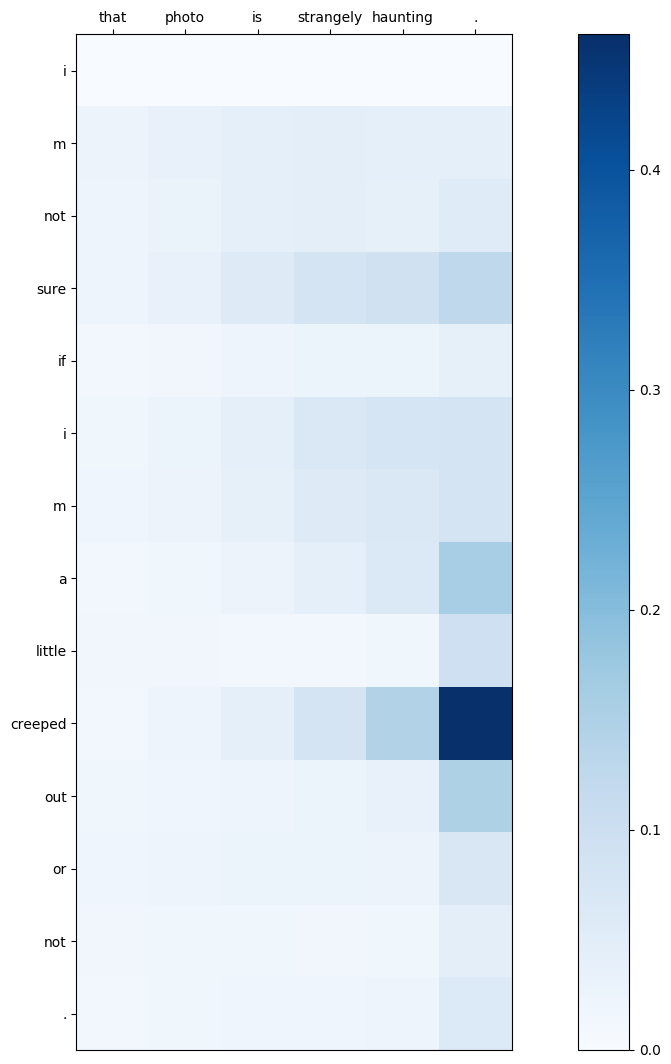
\includegraphics[width = 3in]{img/attention_heatmap_example}}
	\subfigure[Attention weights visualized via a weights overlay]{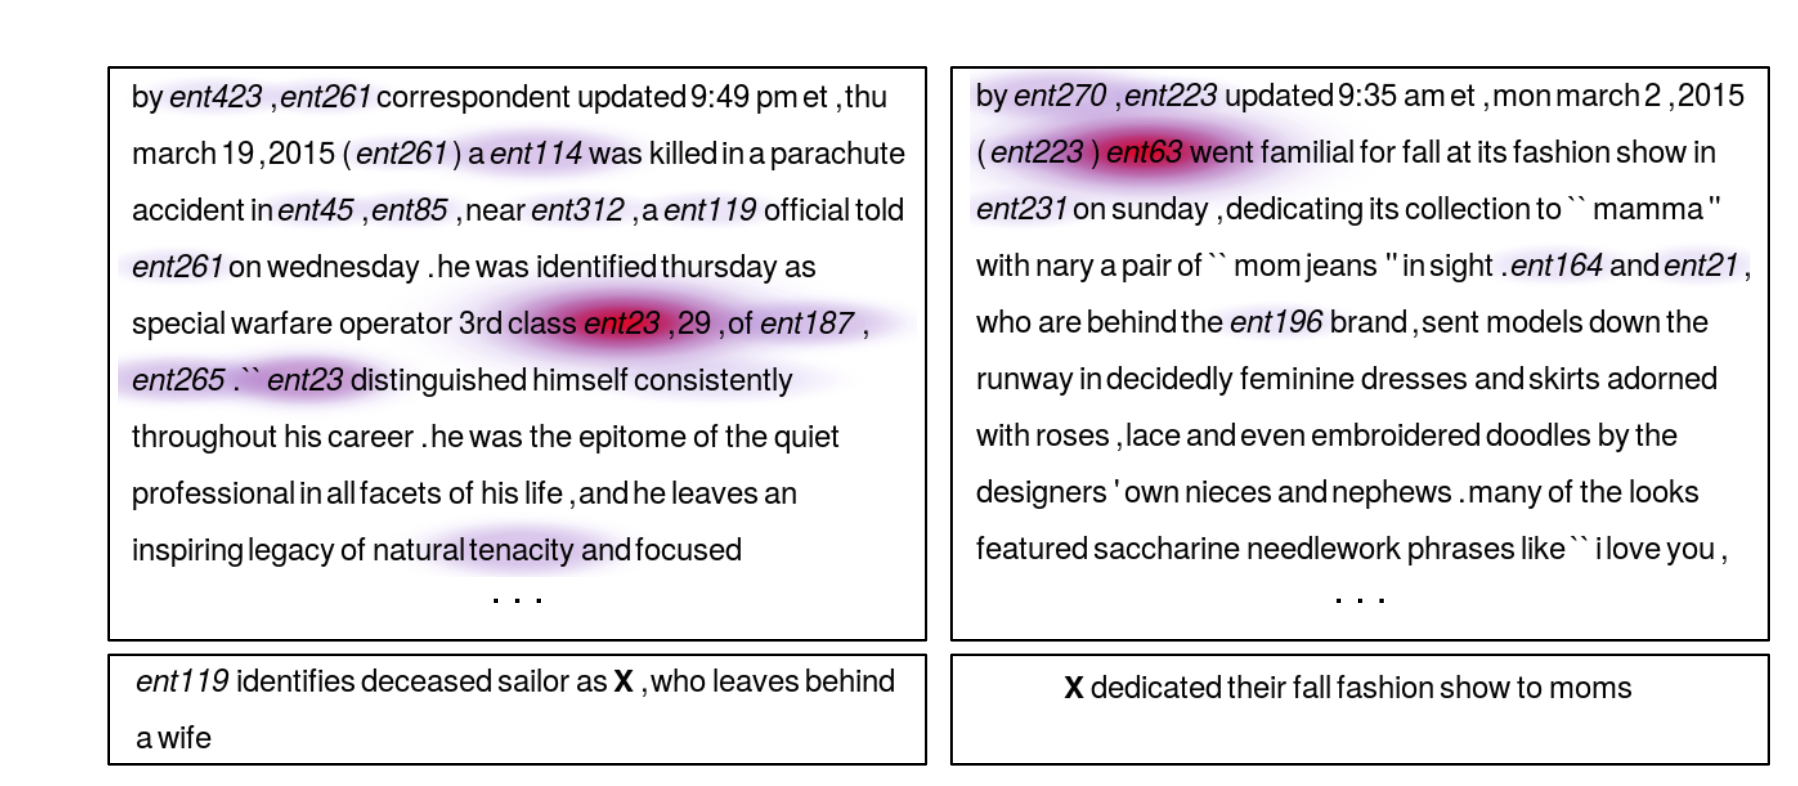
\includegraphics[width = 3in]{img/attention_overlay_example}}
	\caption{Examples of how attention weights can be visualized using heatmaps and overlays.}
	\label{fundamentals:seq2seq:attention_weights_visualization}
\end{figure}

The name \emph{soft}-attention comes from the fact, that this kind of attention mechanism is fully differentiable and hence can be simply plugged into any existing NN architecture. The other kind of of attention is the so-called \emph{hard}-attention mechanism which in contrast selects a random XYZ and because of that, it is not fully differentiable and hence cannot simply be added to an existing system running with back-propagation and gradient-descent.

We have only explained on how soft-attention can be used in a context where we process language. However, the attention mechanism itself originated from the computer vision area !!REFERENZ!!. The mechanism can be adapted to any kind of problem and model, not just computer vision or NLP, as long as the model has any way of accessing the input data.

\paragraph{Decoding Approaches} In the following paragraph, we are going to elaborate on two decoding approaches that we are going to use in our experiments: \emph{greedy} decoding and \emph{beam-search} decoding.

Greedy decoding is the simpler of the two variants. When using it, the output $y_t$ of the model using it is simply the token with the highest probability after the softmax layer has been applied on the last hidden state $h_t$ of the decoder at time $t$. It then goes on by feeding in the hidden state $h_t$ to produce the output token $y_{t+1}$ for the next time step $t+1$. This variant is really simple to implement, but also has its flaws: Since the decoder is working in a local and greedy fashion, it has to take ...

Beam-Search tries to fix or at least minimize this problematic by not only considering a single candidate sequence but instead focuses on the $m$ different sequences, which are most promising. The variable $m$ is called the \emph{beam width} and signifies how much possible candidate sequences are under consideration. The approach itself works by doing the usual computation and process the input sequence with the encoder cell at the beginning. The last hidden state is then passed to the decoder which starts to do the beam search. It begins by using the last hidden state to predict the first word of the output in the same way as the greedy decoder does. It then feeds back in the hidden state of the decoder after the first output token has been generated and generates the next probability distribution over the vocabulary (by using the softmax layer at the end). But now, instead of simply choosing the next token to be the one with the highest probability, the decoder stores the $m$ tokens with the highest probability.

\begin{itemize}
	\item Explain two approaches: Greedy and Beam-Search.
	\item Explain why greedy might not give satisfactory results.
\end{itemize}

\section{Performance Metrics}
In this section, we are going to introduce the main performance metrics used in this thesis to asses the performance of the trained models.

\paragraph{Cross-Entropy Loss} For our model, we are primarily using the \emph{Cross-Entropy} loss function while training. It can be used to measure how well an expected probability distribution $p$ is predicted by a trained model, where the prediction is denoted as $q$. In our case, the probability distribution $p(x)$ is the distribution of the words predicted by the decoder at the time step $t$ and $q(x)$ is the expected distribution for the given sample $x$. The loss function is defined via the following equation where $X$ stands for the whole training dataset:

\begin{equation}
H(p, q) = - \sum_{X} p(x) log_2(q(x))
\end{equation}

In the case of sequence-to-sequence learning, the expected probability is effectively a one-hot encoded vector with a $1$ at the entry of the expected word at time step $t$. This loss function can be used for training a seq2seq model (or any model which predicts probability distributions in a broader sense) and it can then also be used to calculate the perplexity of the model, which we are going to elaborate on below.

\paragraph{Perplexity} The perplexity is another metric for measuring how good a language model will predict the sentences in the test dataset and is closely tied to the cross-entropy loss function. The value of the perplexity can be computed by raising the value of the cross-entropy loss function to the power of $2$. The perplexity can be computed by the following equation:

\begin{equation}
\operatorname{perplexity}(X) = 2^{H(X)} = 2^{- \sum_{X} p(x) log_2(q(x)}
\end{equation}

!!MORE!!

\paragraph{Sent2Vec Similarity} We were seeking for a third performance metric, since the perplexity is simply the result of the loss function raised to the power of $2$. This means, we effectively have one performance metric to use. To fix this problem, we also investigated into using \texttt{Sent2Vec}\footnote{https://github.com/epfml/sent2vec} \cite{Pgj:2017} for measuring the semantic similarity of the sentences generated by the model when testing it after it has been trained. We propose the following way to test the model:

\begin{enumerate}[noitemsep]
	\item Allocate a variable for storing the sum of distances.
	\item Repeat the following steps until all samples in the test set are exhausted:
	\begin{enumerate}[noitemsep]
		\item Create prediction for the given input sentence.
		\item Embed the generated and expected sentences via \texttt{Sent2Vec} to obtain n-dimensional embedding vectors for both of them.
		\item Measure the distance by using the euclidean distance between the embeddings in the n-dimensional vector space.
		\item Add this distance to the sum of distances.
	\end{enumerate}
	\item Divide the sum of distances by the number of samples. This is the final result which can be used as a metric.
\end{enumerate}

This procedure allows us to further analyze the performance of the model by comparing the semantic similarities between the expected and the generated answers. For example, when the expected output sentence is ''I feel good, how about you?'' and the answer generated by the model is ''I'm fine, you?'', the similarity measurement should return a small value since we would expect that this sentences are embedded closely to each other due to the semantic similarity of the content. In contrast, when the output of the model is ''I really love cupcakes'' and the expected is still the same, the similarity measure should become big to signify that there is a large mismatch between the meaning of the expected and generated sentence.

